% Deuxième partie — Pipeline DRAIN + LogBERT + SLM (niveau ingénieur, double diplôme)
% Compiler : pdflatex partie2.tex (figures dans ./figs/)
\documentclass[12pt,a4paper]{report}
\usepackage[utf8]{inputenc}
\usepackage[T1]{fontenc}
\usepackage[french]{babel}
\usepackage{hyperref}
\usepackage{graphicx}
\usepackage{booktabs}
\usepackage{amsmath}
\usepackage{caption}
\usepackage{geometry}
\usepackage{setspace}
\usepackage{float}
\usepackage{enumitem}
\usepackage{tikz}
\geometry{margin=2.5cm}
\hypersetup{colorlinks=true,linkcolor=black,citecolor=black,urlcolor=blue}
\graphicspath{{figs/}}
\onehalfspacing
\setlength{\parskip}{0.6em}
\setlength{\parindent}{0pt}
\raggedbottom
\setlength{\textfloatsep}{20pt}
\setlength{\intextsep}{20pt}
\setlist[itemize]{itemsep=0.4em, topsep=0.4em}
\setlist[enumerate]{itemsep=0.4em, topsep=0.4em}

\begin{document}

% ================= PAGE DE GARDE =================
\begin{titlepage}
\begin{center}
% Bandeau logos : entreprise + établissements du double diplôme
\begin{tabular}{cccc}

\includegraphics[height=1cm]{Logo-Worldline-Pepper-Horizontal-rgb.png} &

\includegraphics[height=1cm]{logo_politehnica.png} &

\includegraphics[height=1cm]{acs_logo.png} &

\includegraphics[height=1cm]{logo-3il.png} \\
{\small Worldline} & {\small UNST Politehnica Bucarest} & {\small ACS} & {\small 3iL Ingénieurs} \\
\end{tabular}
\vspace{0.6cm}

{\large UNIVERSITÉ POLYTECHNIQUE DE BUCAREST \par}
{\normalsize Faculté d'Automatique et d'Informatique — Master 2 Intelligence Artificielle \par}
\vspace{0.2cm}
{\large 3iL INGÉNIEURS — Double diplôme \par}
\vspace{0.4cm}
\rule{\linewidth}{1pt}
\vspace{0.4cm}
{\LARGE \textbf{Diagnostic des logs par IA hybride} \par}
\vspace{0.2cm}
{\Large Pipeline DRAIN~+~LogBERT~+~SLM pour la détection d'anomalies et la réduction du MTTR \par}
\vspace{0.2cm}
{\large Mémoire de double diplôme Master IA — UPB Bucarest / 3iL Ingénieurs \par}
\rule{\linewidth}{1pt}
\vspace{0.6cm}
{\large Mémoire présenté par \par}
{\Large \textbf{SYLLA Abdou Lahat} \par}
\vspace{0.4cm}
\begin{tabular}{ll}
Année universitaire : & 2025/2026 \\
Entreprise d'accueil : & Worldline — Pôle Trading \& Financial Information (TFI) \\
Équipe : & Client Delivery 2 \\
Encadrants entreprise : & Ludovic Charvoz, Doreen Lucky Tchoupe Soh \\
\end{tabular}
\vspace{0.6cm}
\begin{tabular}{ll}
\hline
Protocole : & train normal-only, sélection sur validation, test verrouillé \\
Données : & HDFS complet, 575\,061 sessions, 11\,175\,629 événements \\
Référence : & Guo et al., LogBERT, IJCNN 2021 \\
Modèle retenu : & V2 $m{=}0{,}75$, $g{=}8$, $r{=}0{,}04$ \\
\hline
\end{tabular}
\vfill
{\normalsize Document de travail — figures issues du run Kaggle GPU T4 (dépôt officiel LogBERT, commit \texttt{a845e61}). \par}
\end{center}
\end{titlepage}

\tableofcontents
\newpage

\chapter{Diagnostic des logs par IA hybride : pipeline DRAIN~+~LogBERT~+~SLM}

\section{Introduction générale}

Ce rapport traite d'une problématique d'entreprise unique : diagnostiquer vite et à coût maîtrisé des incidents noyés dans des flux de logs bancaires massifs, sans sortir les données du réseau privé. Mené en alternance chez Worldline (équipe Client Delivery~2, pôle TFI) et dans le cadre du double diplôme Master IA (Université Polytechnique de Bucarest / 3iL Ingénieurs), il articule retour d'expérience opérationnel et travaux de recherche appliquée : un pipeline hybride où DRAIN structure les logs, LogBERT détecte statistiquement, et un SLM contraint explique pour l'astreinte. Le plan suit ce fil : présentation de l'entreprise, formulation de la problématique, état de l'art, architecture et protocole, apprentissage, résultats sur test verrouillé, inférence et applicabilité en production, puis conclusion.

\section{Présentation de l'entreprise d'accueil}

Worldline, fournisseur européen de services de paiement (4\textsuperscript{e} rang mondial), opère depuis Paris La Défense dans plus de 50~pays avec plus de 18\,000~collaborateurs. Mon alternance s'est déroulée dans l'équipe \textbf{Client Delivery~2}, rattachée au pôle \textbf{Trading \& Financial Information (TFI)} de la branche Financial Services : hébergement spécialisé et maintien en condition opérationnelle d'infrastructures critiques pour des clients bancaires (Copartis, CommerzBank, Boursorama), sur cloud privé maison et périmètres on-premise.

Seul le contexte Copartis est mobilisé dans ce mémoire, comme motivation du sujet IA : $\sim$172~millions de lignes de logs mensuelles hors INFO/WARN (66~logs/s en moyenne, pics à 2\,506~logs/s sur 30~jours) et un incident cascade côté CRM CommerzBank ($\sim$4\,600~lignes, trois composants) relevant du socle (librairie Oracle manquante, saturation mémoire, résolution d'hôte base de données). C'est ce besoin --- qualifier vite un incident dans des flux massifs, sans sortir les données du réseau privé --- qui motive le pipeline DRAIN~+~LogBERT~+~SLM étudié dans le cadre du double diplôme Master IA (UPB Bucarest / 3iL).

\section{Introduction de la réflexion}

\subsection{Contexte opérationnel et réalité de la gestion des logs}

L'exploitation quotidienne du périmètre (présenté ci-dessus) repose sur des règles à seuils et l'expertise de l'astreinte. Deux limites vécues motivent ce travail : (i)~les seuils manquent les dégradations lentes et noient l'astreinte sous des cascades d'alertes corrélées ; (ii)~face à une cascade sans cause évidente, imputer l'incident au socle ou au code client exige un tri manuel de milliers de lignes --- comme lors de l'incident CRM, résolu en isolant trois causes socle par analyse assistée (LibreChat interne). D'où l'objectif : passer du tri manuel à une détection statistique couplée à une explication contrainte.

\subsection{Chronologie et genèse du projet}

Semestre Master~2 IA à l'Université Polytechnique de Bucarest (S1 2025/2026) : attention~\cite{vaswani2017attention}, VAE~\cite{kingma2013vae}, BERT~\cite{devlin2018bert}. Retour en entreprise le 16~février~2026 : le projet monolithique initial (Ludovic Charvoz, Doreen Lucky Tchoupe Soh) était abandonné pour des verrous de volumétrie, d'interfaçage, de confidentialité et de coût. D'où la proposition d'une architecture frugale, modulaire et souveraine, objet de cette partie.

\subsection{Problématique}

\begin{quote}
\emph{Face à l'explosion de la volumétrie des logs et aux contraintes financières du cloud, comment l'hybridation DRAIN + LogBERT + SLM réduit-elle significativement le MTTR tout en garantissant une soutenabilité FinOps ?}
\end{quote}

Exigences d'ingénieur : reproductibilité, protocole sans fuite test, décision traçable, coût borné, données confinées au réseau privé.

\section{État de l'art}

\subsection{Supervision à seuils et fatigue d'alerte}

Les règles à seuils (ex.\ \texttt{LBHealthCheckServerDown} : backend HAProxy DOWN $>$ 2~min) détectent les pannes franches mais manquent les dégradations lentes et produisent des avalanches d'alertes corrélées qui désensibilisent l'astreinte~\cite{ndichu2026}. Les approches classiques de parsing (Drain~\cite{he2017drain}, Spell, IPLoM) et de détection (DeepLog~\cite{du2017deeplog}, LogAnomaly~\cite{meng2019loganomaly}) sont résumées par Zhu et al.~\cite{zhu2019tools} et le benchmark LogHub~\cite{he2020loghub}.

\subsection{Impasse du tout-LLM}

Fenêtre de contexte saturée par les flux continus, coût quadratique de l'attention, dilution du signal et hallucinations factuelles inacceptables en banque~\cite{ji2023hallucination}. Les petits modèles instructionnels (Qwen2.5~\cite{qwen2025}, Llama-3~\cite{llama3}) changent l'équation seulement s'ils n'interviennent qu'en aval d'un filtrage statistique strict.

\subsection{DRAIN et LogBERT}

DRAIN~\cite{he2017drain} route chaque log par longueur et préfixe dans un arbre à profondeur fixe et extrait le template en masquant les variables. La Figure~\ref{fig:drain} illustre ce passage du log brut au template : les parties variables (identifiants, adresses, temps) sont remplacées par des jokers, et chaque message est réduit à sa signature structurelle.

\begin{figure}[htbp]
\centering
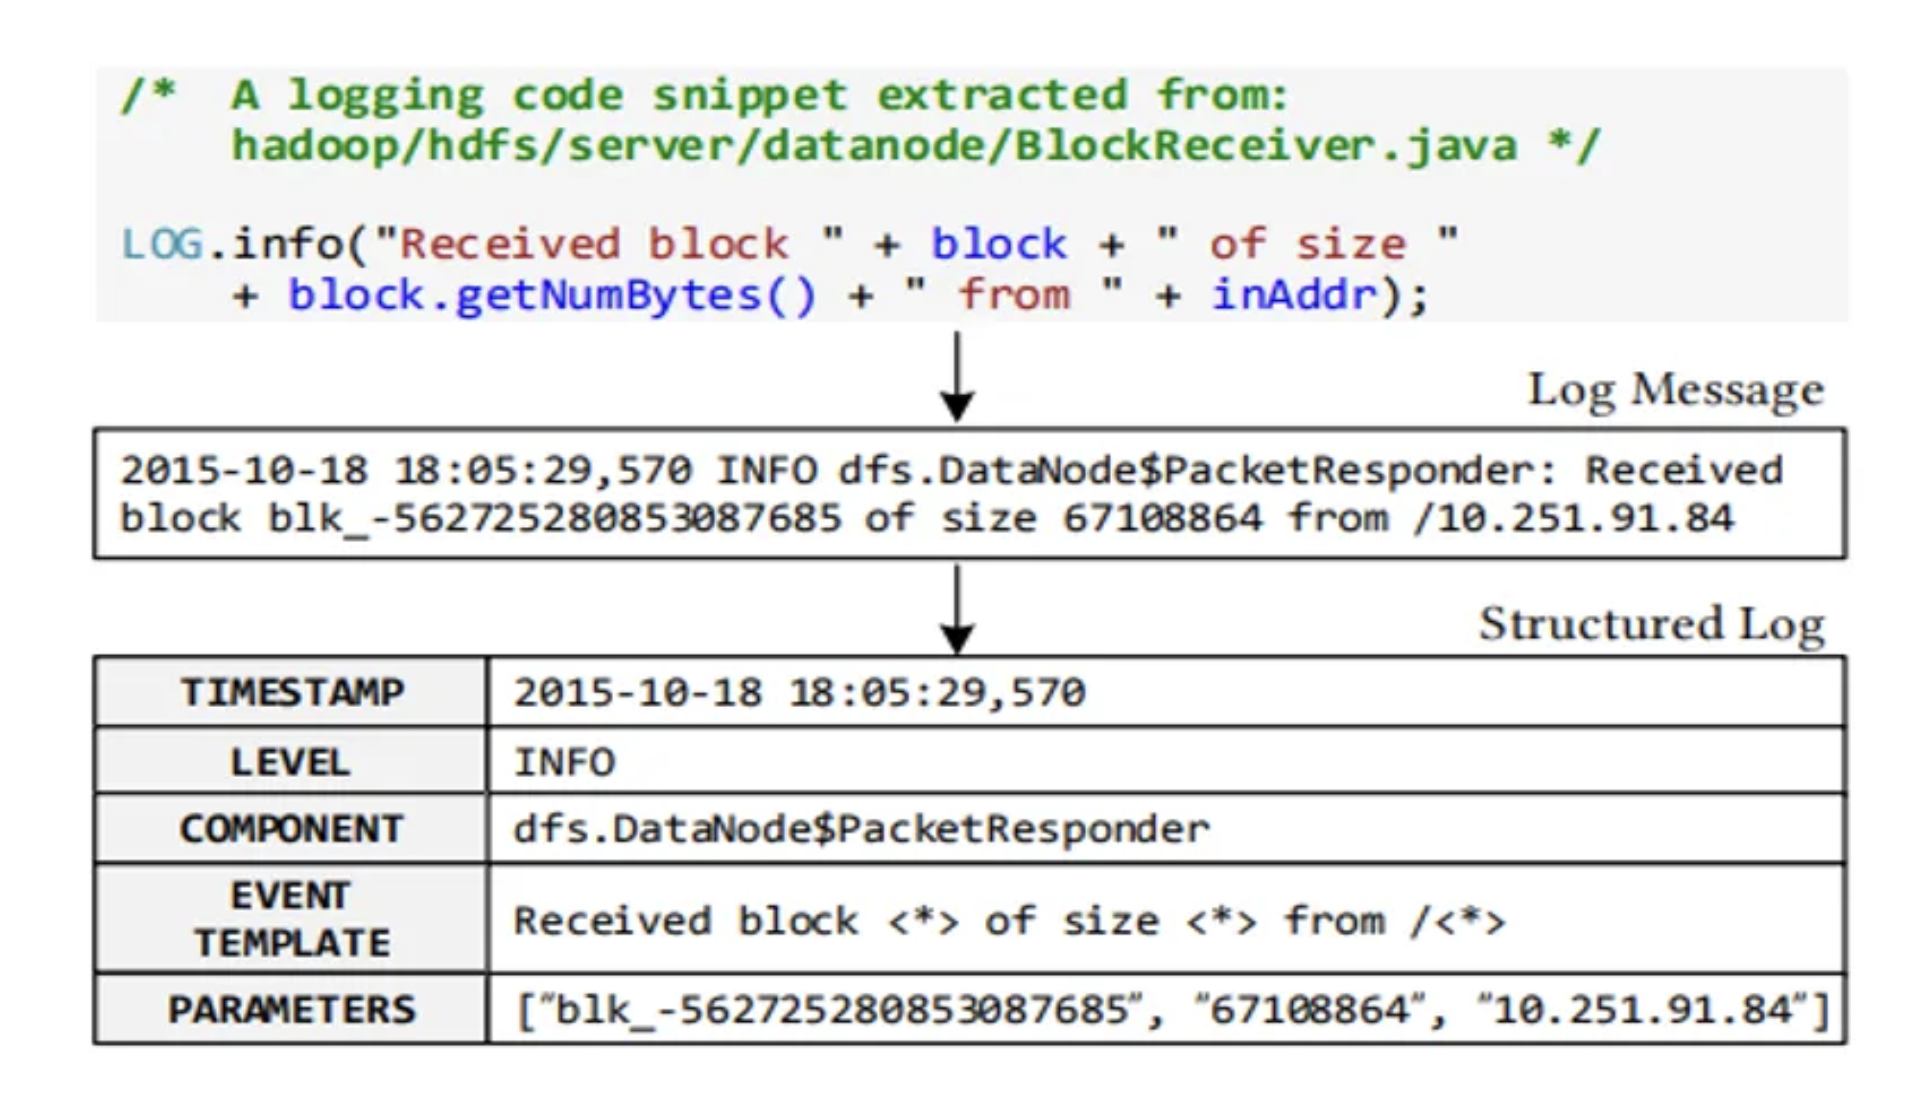
\includegraphics[width=0.95\linewidth]{drain-illustration.png}
\caption{Parsing DRAIN : du log brut au template structuré (les variables sont masquées, le squelette fixe est conservé).}
\label{fig:drain}
\end{figure}

LogBERT~\cite{guo2021logbert} entraîne un Transformer sur séquences de clés avec MLKP (prédiction de clés masquées, ratio $m$) et VHM (compacité des normaux). Score paper-style : pour chaque position masquée, erreur si l'observé est hors top-$g$ ; session anormale si proportion d'erreurs $> r$. Le même $m$ sert en entraînement et en inférence.

\subsection{Comparaison aux méthodes existantes (SOTA du papier LogBERT)}

Le papier LogBERT~\cite{guo2021logbert} évalue sur HDFS, BGL et Thunderbird six baselines représentatives de trois familles : méthodes à vecteurs de comptage + détecteur classique (\textbf{PCA}~\cite{xu2009detecting}, \textbf{One-Class SVM}~\cite{scholkopf2001estimating}, \textbf{Isolation Forest}~\cite{liu2008isolationforest}, \textbf{LogCluster}~\cite{lin2016logcluster}) et réseaux récurrents (\textbf{DeepLog}~\cite{du2017deeplog}, \textbf{LogAnomaly}~\cite{meng2019loganomaly}). Toutes utilisent Drain~\cite{he2017drain} pour le parsing ; PCA/OCSVM/iForest/LogCluster sont évalués via Loglizer~\cite{he2016experience}. Le Tableau~\ref{tab:sota-hdfs} reprend les chiffres HDFS du papier (Table~2, moyennes sur test à 553\,366~normales / 10\,647~anomalies).

\begin{table}[H]
\centering
\begin{tabular}{lccc}
\toprule
Méthode & Precision & Recall & F1 \\
\midrule
PCA & 0,0589 & 1,0000 & 0,1112 \\
Isolation Forest & 0,5360 & 0,6941 & 0,6049 \\
OCSVM & 0,0254 & 1,0000 & 0,0495 \\
LogCluster & 0,9926 & 0,3708 & 0,5399 \\
DeepLog & 0,8844 & 0,6949 & 0,7734 \\
LogAnomaly & 0,9415 & 0,4047 & 0,5619 \\
\textbf{LogBERT (article)} & \textbf{0,8702} & \textbf{0,7810} & \textbf{0,8232} \\
\bottomrule
\end{tabular}
\caption{État de l'art sur HDFS d'après Guo et al. (2021), Table~2. Source : \texttt{2103.04475v1.pdf}.}
\label{tab:sota-hdfs}
\end{table}

Lecture : les méthodes à comptage sacrifient l'ordre temporel (PCA/OCSVM à recall 1,0 mais précision quasi nulle) ; LogCluster monte en précision mais manque la moitié des anomalies ; DeepLog et LogAnomaly confirment l'apport du séquentiel, avec le meilleur F1 classique à 0,7734 (DeepLog). LogBERT (0,8232) les dépasse avec une balance précision/recall supérieure. L'ablation du papier (Table~3) éclaire ce gain : MLKP seule donne 0,7754 / 0,7865 / 0,7809, VHM seule 0,0243 / 0,3917 / 0,0458, et la combinaison MLKP+VHM 0,8702 / 0,7810 / 0,8232 --- la VHM apporte +4,2~pts de F1 sur HDFS aux séquences courtes (longueur moyenne 19), là où son apport est marginal sur BGL/Thunderbird aux séquences longues. C'est ce socle que notre protocole V1/V2 reprend à l'identique (même scoring top-$g$/$r$, même $m$ en train et inférence), avant d'en tester la sensibilité à $m$.

\textbf{Baseline article (Guo et al., 2021, HDFS) : Precision 87,02\,\%, Recall 78,10\,\%, F1 82,32\,\%.} Référence indicative, non appariée : split différent, seuil officiel réglé sur le test, 4 couches dans le code contre 2 décrites. Dépôt : \url{https://github.com/HelenGuohx/LogBERT.git}, commit \texttt{a845e61}~\cite{logbert-repo}.

\section{Architecture du pipeline}

\begin{figure}[htbp]
\centering
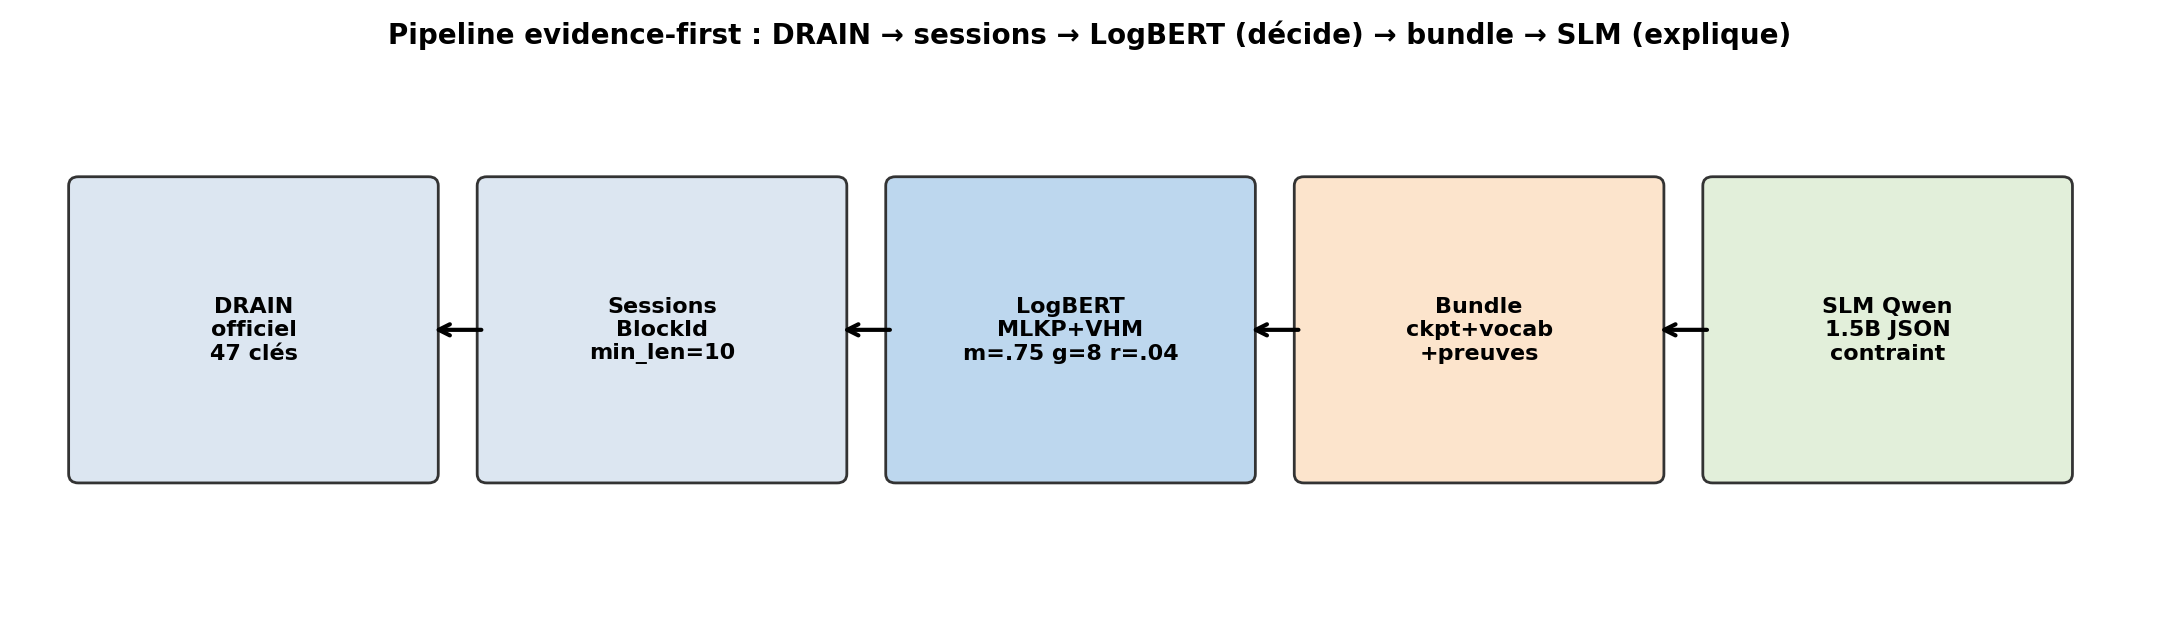
\includegraphics[width=0.95\linewidth]{fig_pipeline.png}
\caption{Architecture evidence-first en entonnoir. LogBERT décide ; la politique déterministe filtre ; le SLM explique.}
\label{fig:pipeline}
\end{figure}

Cinq étages : (1)~parsing DRAIN officiel $\rightarrow$ 47 clés ; (2)~sessionnisation par \texttt{BlockId}, \texttt{min\_len}=10 ; (3)~LogBERT MLKP+VHM ; (4)~bundle AIOps (\texttt{best\_bert.pth}, \texttt{vocab.pkl}, mapping Drain, \texttt{inference.py}, manifeste) avec API sur séquences d'\texttt{EventId} ; (5)~SLM Qwen2.5-1.5B-Instruct en JSON contraint (résumé ingénieur, lecture LogBERT, chaîne causale probable, incertitudes, actions P1--P3, événements cités). Le SLM ne re-décide jamais ; toute action libre est interdite (catalogue fini + injection déterministe des paramètres).
, avec un seul sens de lecture : plus on avance vers la droite de la Figure~\ref{fig:pipeline}, moins il y a de données et plus le contenu est qualifié.

\section{Protocole expérimental}

Kaggle GPU T4. Données HDFS\_v1 (Zenodo 8196385, MD5 \texttt{76a24b4d9a6164d543fb275f89773260}), labels logpai/loglizer. \textbf{Train normal-only} : 4\,855 sessions (shuffle seed 20 du script officiel). \textbf{Validation} : 55\,336 normales / 2\,139 anomalies. \textbf{Test verrouillé} : 498\,032 / 8\,508 (prévalence 1,68\,\%), \texttt{BlockId} disjoints, 575\,061 sessions et 11\,175\,629 événements au total (médiane 19, p95 28). Vocabulaire issu du seul train. Sélection $m,g,r$ sur validation (projection à la prévalence de référence) ; métriques test à la prévalence réelle + Wilson 95\,\%.

Grille V2 : $m \in \{0{,}50, 0{,}65, 0{,}75\}$, $g \in \{1,\dots,15\}$, $r \in [0,0{,}80]$ pas 0,01, un seed. V1 = baseline officielle $m{=}0{,}65,g{=}6,r{=}0$. Correctifs sans changement modèle : \texttt{torch.\_six}, \texttt{np.float/int/Inf}, ragged \texttt{dtype=object}, pandas 2.2.3 / NumPy 2.x.

\section{Apprentissage : courbes train / validation}

\begin{figure}[htbp]
\centering
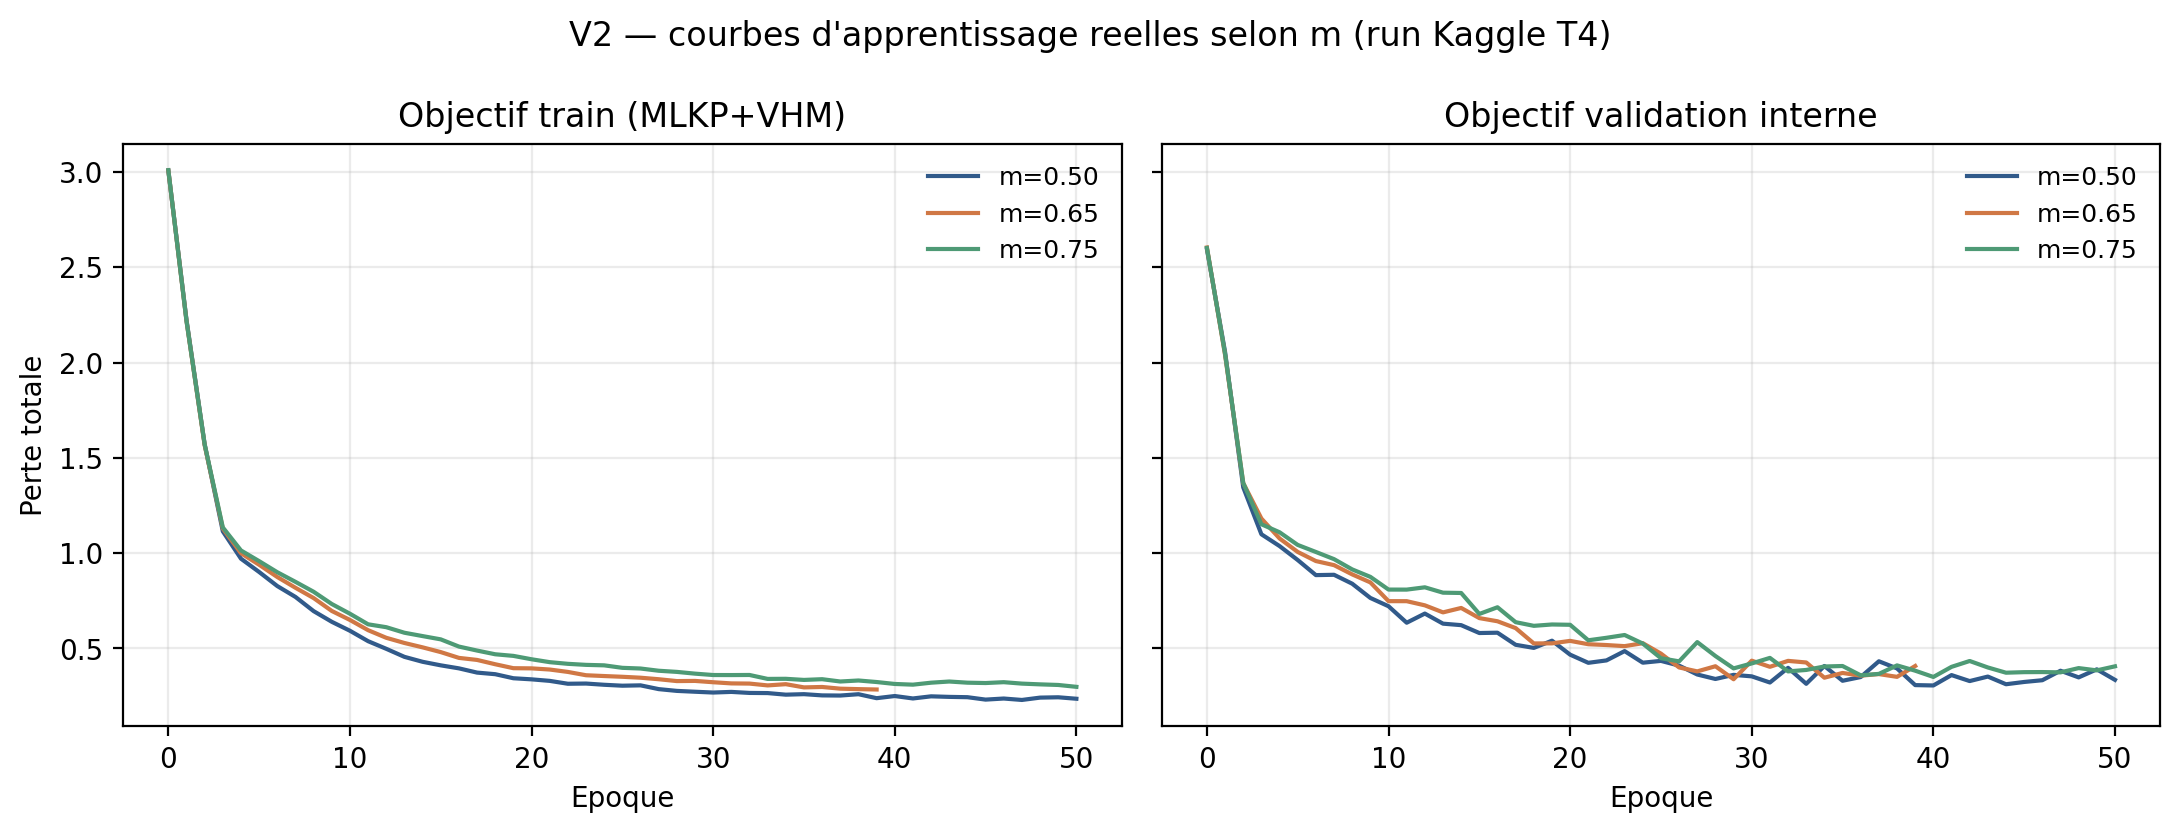
\includegraphics[width=0.95\linewidth]{fig_loss_train_val.png}
\caption{Courbes réelles de l'objectif total MLKP+VHM (run Kaggle). Train : 0,2356 ($m{=}0{,}50$), 0,2842 ($m{=}0{,}65$, arrêt précoce à 40 époques), 0,2982 ($m{=}0{,}75$) ; validation interne : 0,3348 / 0,4075 / 0,4058. La perte minimale ($m{=}0{,}50$) ne donne pas la meilleure détection.}
\label{fig:loss}
\end{figure}

la chute initiale est commune aux trois courbes et l'écart train/validation reste stable ; le triplet $m{=}0{,}75,g{=}8,r{=}0{,}04$ maximise le F1 validation (0,8493), avec un F1 test à 0,8314 ($-$1,8~pt, généralisation saine).

Lecture d'ingénieur : convergence rapide (chute de $\sim$3,0 à $<$1,0 en $\sim$5 époques), puis plateau ; écart train/validation stable ($\sim$0,10), sans divergence explosive grâce au plafonnement NLL ; early stopping effectif pour $m{=}0{,}65$. Surtout, \textbf{le meilleur MLKP n'est pas le meilleur détecteur} : la sélection se fait sur F1 validation, pas sur la perte (Figure~\ref{fig:selection}).

\begin{figure}[htbp]
\centering
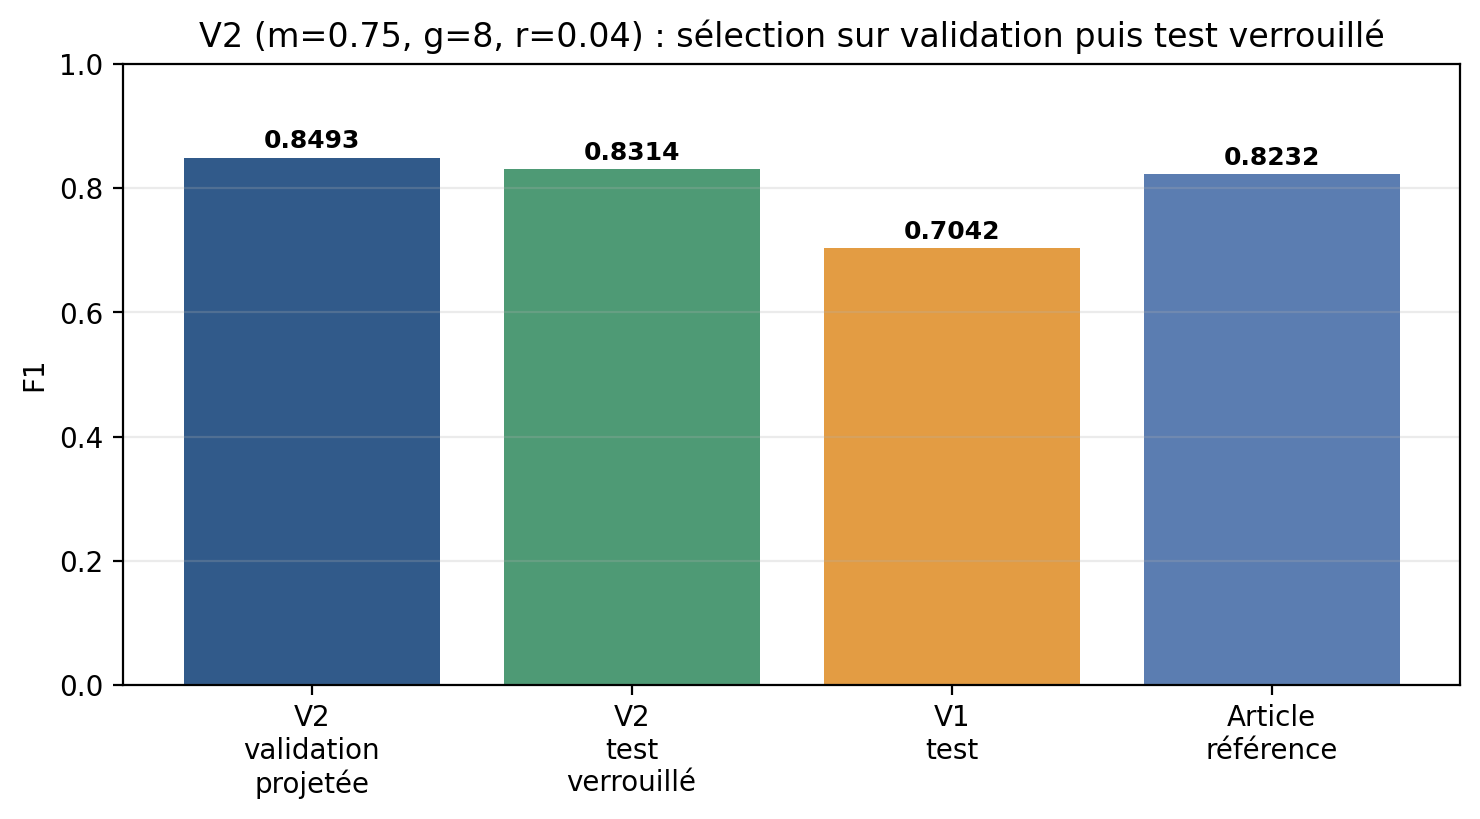
\includegraphics[width=0.85\linewidth]{fig_selection_m.png}
\caption{Sélection validation-only puis test verrouillé : F1 validation projetée 0,8493 pour le triplet $m{=}0{,}75,g{=}8,r{=}0{,}04$ (précision projetée 0,8677, recall 0,8317), F1 test 0,8314. Le test n'est scoré qu'après gel.}
\label{fig:selection}
\end{figure}

\section{Résultats sur test verrouillé}

Les Figures~\ref{fig:comparaison} et~\ref{fig:confusion} encadrent le Tableau~\ref{tab:comparaison}.

\begin{figure}[htbp]
\centering
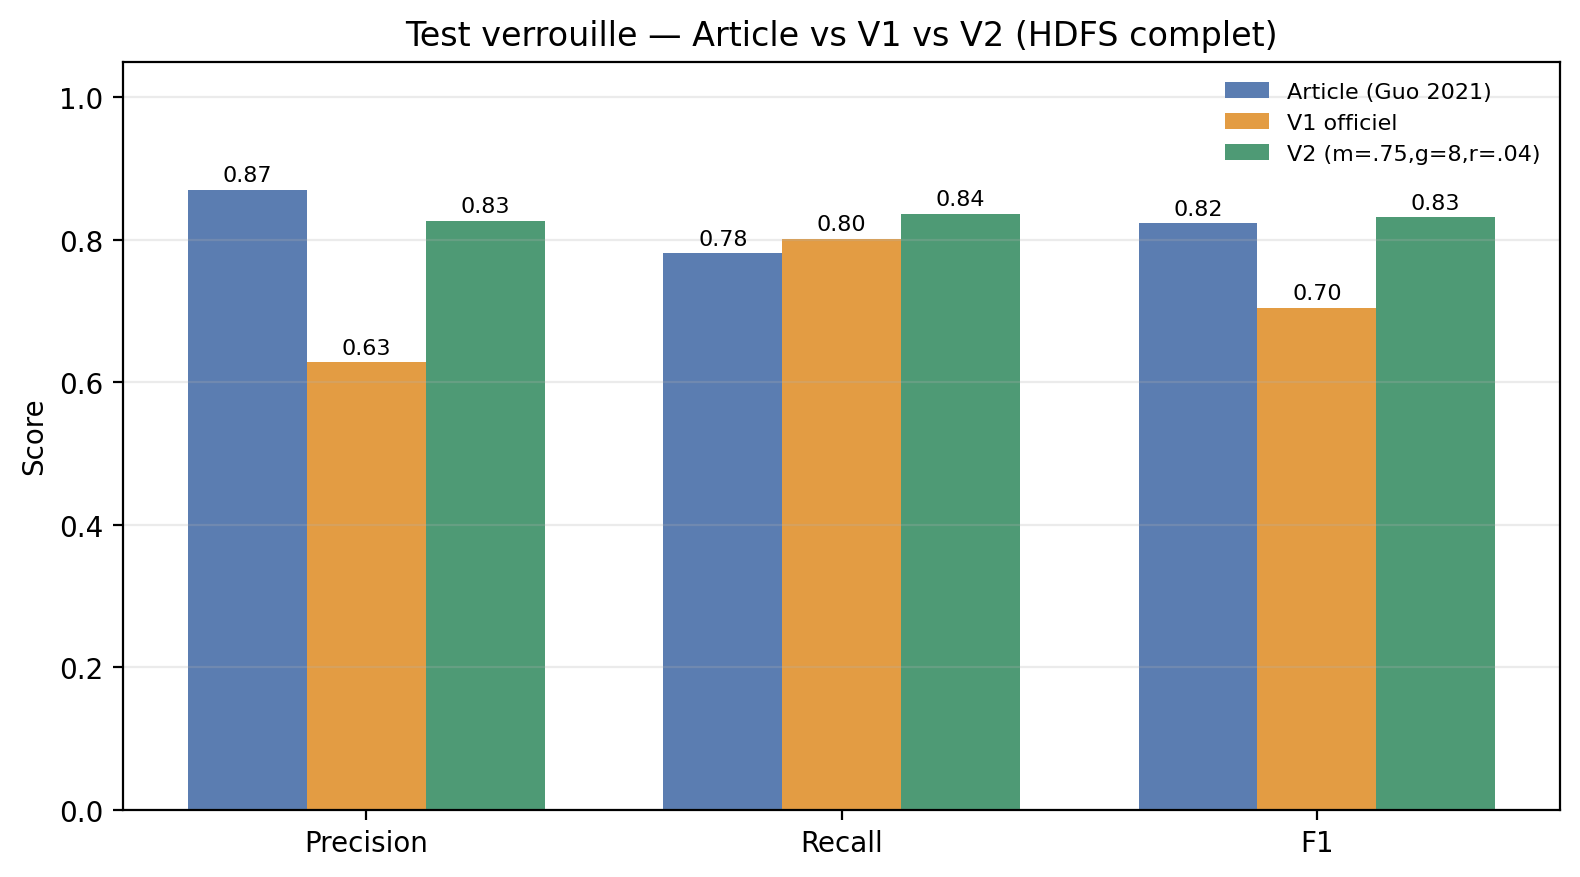
\includegraphics[width=0.95\linewidth]{fig_comparaison.png}
\caption{Test verrouillé HDFS complet : article (référence non appariée) vs V1 officielle vs V2.}
\label{fig:comparaison}
\end{figure}

\begin{table}[h]
\centering
\caption{Comparaison test verrouillé. Article : référence indicative.}
\label{tab:comparaison}
\renewcommand{\arraystretch}{1.35}
\begin{tabular}{lccccc}
\toprule
Version & Precision & Recall & F1 & ROC-AUC & PR-AUC \\
\midrule
Article HDFS & 0,8702 & 0,7810 & 0,8232 & --- & --- \\
V1 ($m{=}0{,}65,g{=}6,r{=}0$) & 0,6278 & 0,8017 & 0,7042 & 0,8979 & 0,6338 \\
\textbf{V2 ($m{=}0{,}75,g{=}8,r{=}0{,}04$)} & \textbf{0,8267} & \textbf{0,8362} & \textbf{0,8314} & \textbf{0,9235} & \textbf{0,7051} \\
\bottomrule
\end{tabular}
\end{table}

\begin{figure}[htbp]
\centering
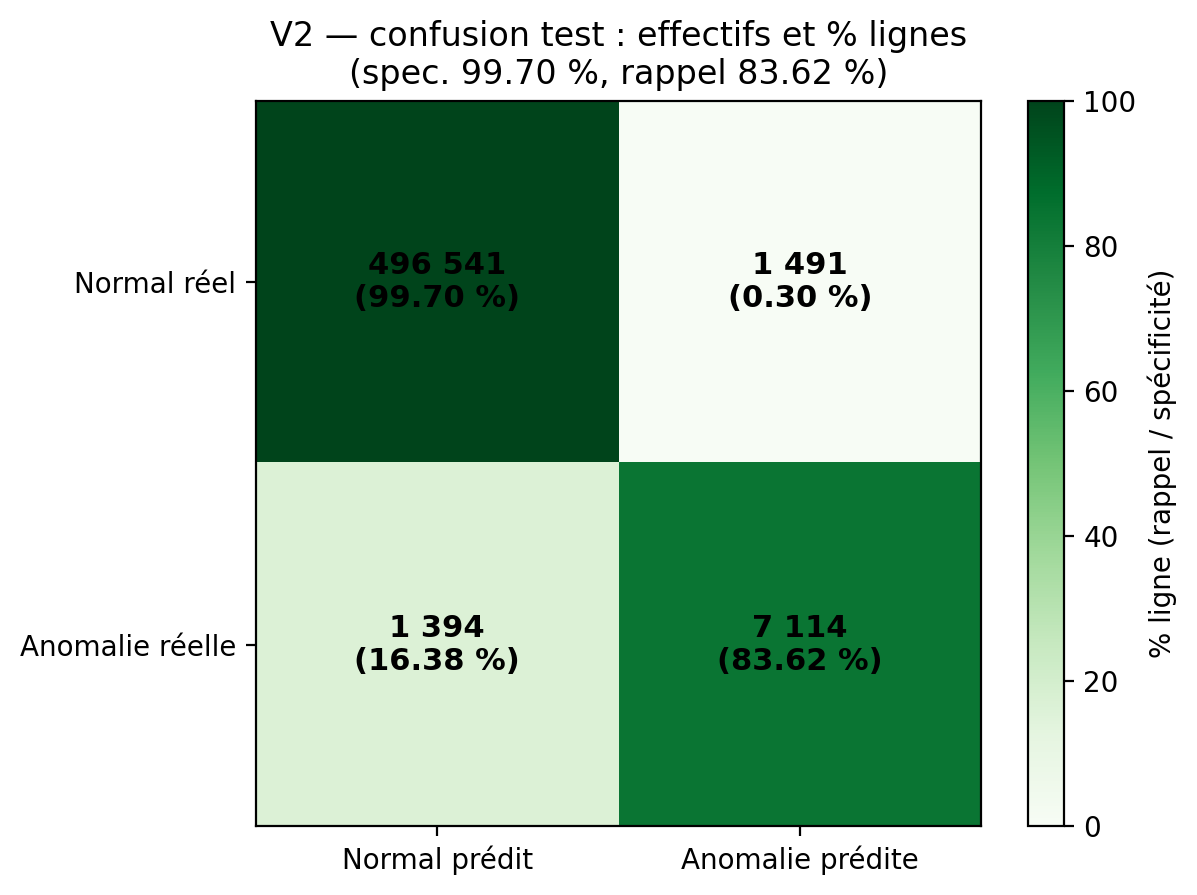
\includegraphics[width=0.75\linewidth]{fig_confusion.png}
\caption{Matrice V2 en effectifs et \% lignes : 496\,541 normaux bien classés (99,70\,\%) et 7\,114 anomalies détectées (83,62\,\%) ; 1\,491 FP (0,30\,\%) et 1\,394 FN (16,38\,\%).}
\label{fig:confusion}
\end{figure}

Détail V2 : Precision IC95 [0,8186 ; 0,8346], Recall IC95 [0,8281 ; 0,8439], FPR 0,0030, Accuracy 0,9943, \textbf{Balanced accuracy 0,9166}, Specificity 0,9970. Écart validation $\rightarrow$ test : 0,8493 $\rightarrow$ 0,8314 ($-$1,8~pt), généralisation saine.

\textbf{Lecture :} V2 bat V1 de +19,9~pts (P), +3,4~pts (R), +12,7~pts (F1), FPR $\div$2,7. Face à l'article : R +5,5~pts, F1 +0,8~pt, P $-$4,35~pts = \textbf{dépassement partiel}. Un seul seed : insuffisant pour revendiquer une supériorité robuste (exiger 3--5 seeds, moyenne $\pm$ écart-type).

\section{Généralisation BGL et rigueur multi-seed (V3)}

Même protocole que V2 (dépôt officiel \texttt{a845e61}, scoring paper-style, train normal-only, sélection sur validation, test verrouillé), appliqué à \textbf{BGL} : 4,7~millions de messages BlueGene/L, fenêtres glissantes 5~min / pas 1~min (longueur moyenne $\sim$562 contre $\sim$19 pour HDFS), shuffle seed~12, \texttt{train\_ratio=0.4}. Split : train 6\,681~normales ; validation 1\,010 / 535 ; test 9\,053 / 2\,091 (prévalence 18,76\,\%). Vocabulaire train-only : 185~clés. Grille $m \in \{0{,}35, 0{,}50, 0{,}65\}$ autour du défaut officiel $0{,}50$ ; seeds 1234/2026/999 à splits figés (seules l'initialisation, l'entraînement et le masquage varient).

\begin{figure}[htbp]
\centering
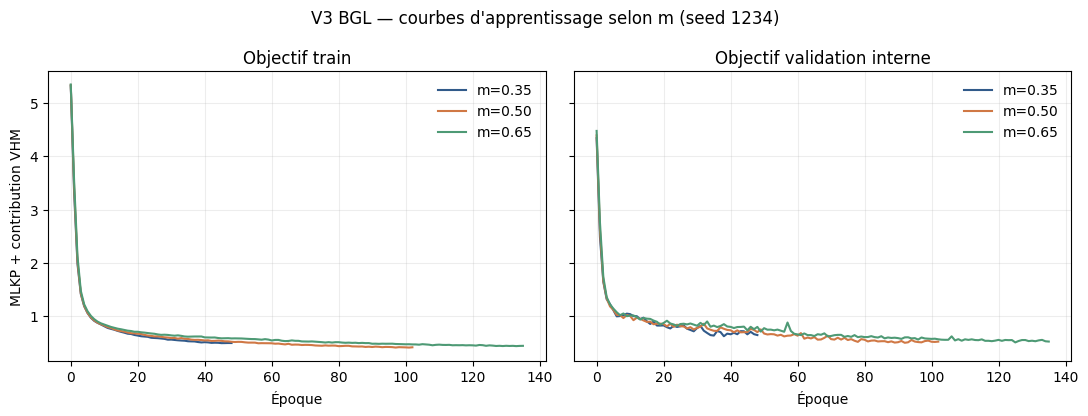
\includegraphics[width=0.95\linewidth]{fig_bgl_loss.png}
\caption{V3 BGL — courbes MLKP+VHM selon $m$ : 49 époques ($m{=}0{,}35$), 103 ($m{=}0{,}50$), 136 ($m{=}0{,}65$). Arrêt précoce effectif, sans divergence.}
\label{fig:bgl-loss}
\end{figure}

Sélection Phase A (seed~1234) : \textbf{$m{=}0{,}50,g{=}15,r{=}0{,}01$} (F1 validation projetée 0,9119, écart validation $\rightarrow$ test $-0{,}2$~pt). Test verrouillé par seed (Tableau~\ref{tab:bgl-seeds}, Figure~\ref{fig:bgl-diag}).

\begin{table}[H]
\centering
\caption{V3 BGL, test verrouillé par seed ; seuils gelés sur validation.}
\label{tab:bgl-seeds}
\renewcommand{\arraystretch}{1.35}
\begin{tabular}{lcccccc}
\toprule
Seed & Precision & Recall & F1 & FPR & ROC-AUC & PR-AUC \\
\midrule
1234 & 0,9046 & 0,9158 & 0,9102 & 0,0223 & 0,9595 & 0,9189 \\
2026 & 0,8979 & 0,9168 & 0,9072 & 0,0241 & 0,9595 & 0,9187 \\
999 & 0,9112 & 0,9173 & 0,9142 & 0,0207 & 0,9597 & 0,9183 \\
\midrule
Moy. ± std (n=3) & 0,9045±0,0066 & 0,9166±0,0007 & 0,9105±0,0035 & 0,0223±0,0017 & 0,9596±0,0001 & 0,9187±0,0003 \\
Article BGL & 0,8940 & 0,9232 & 0,9083 & --- & --- & --- \\
\bottomrule
\end{tabular}
\end{table}

\begin{figure}[htbp]
\centering
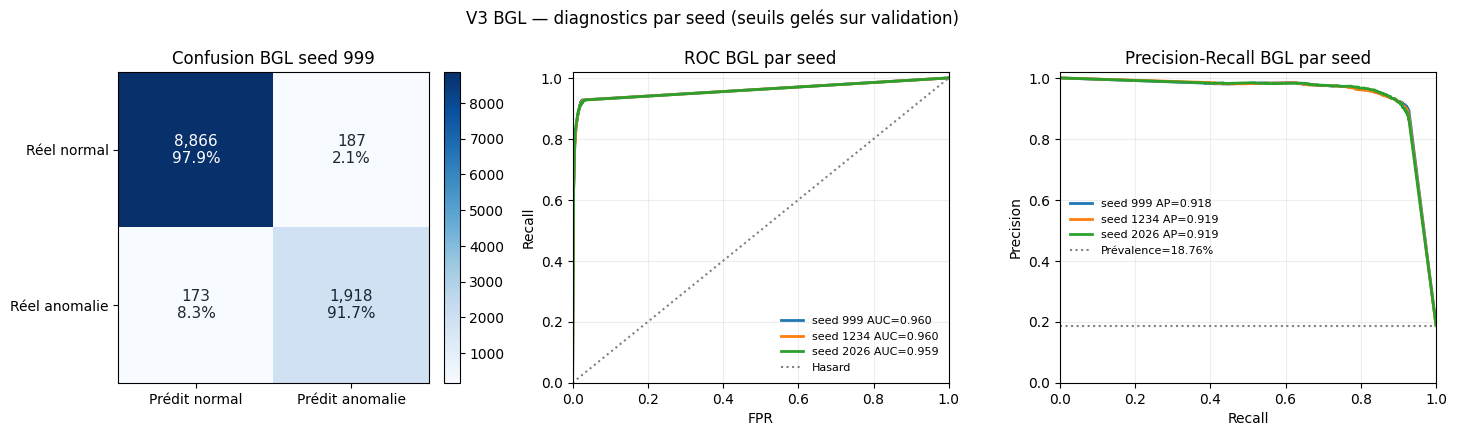
\includegraphics[width=0.95\linewidth]{fig_bgl_diag.png}
\caption{V3 BGL — confusion du meilleur seed (999), ROC et Precision-Recall par seed (seuils gelés).}
\label{fig:bgl-diag}
\end{figure}

\textbf{Lecture :} face au papier BGL (89,40 / 92,32 / 90,83) : P $+$1,05~pt, R $-$0,66~pt, F1 $+$0,22~pt, soit moins que l'écart-type inter-seed ($\pm$0,35) : \textbf{match, pas dépassement}. Le multi-seed interdit ici une revendication abusive — exactement son rôle. Stabilité remarquable (recall $\pm$0,0007, ROC $\pm$0,0001).

\begin{figure}[htbp]
\centering
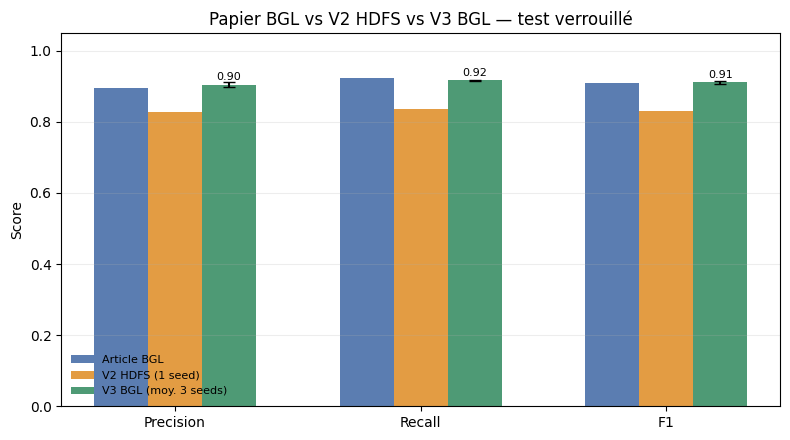
\includegraphics[width=0.95\linewidth]{fig_bgl_cross.png}
\caption{Papier BGL vs V2 HDFS (1~seed) vs V3 BGL (moy. 3~seeds). Les précisions ne sont pas comparables entre datasets (prévalences 18,76\,\% vs 1,68\,\%).}
\label{fig:bgl-cross}
\end{figure}

\textbf{Enseignement principal :} le $m$ optimal suit la longueur des séquences — HDFS ($\sim$19~tokens) voulait $m{=}0{,}75$, BGL ($\sim$562~tokens) confirme le défaut officiel $m{=}0{,}50$ (qui masque déjà $\sim$280~positions par session). L'ablation V2/V3 forme ainsi un résultat unifié plutôt que deux réglages ad hoc. Reste la symétrie : Phase~C (seeds HDFS supplémentaires sur $m{=}0{,}75$) pour la même rigueur côté HDFS.

\section{Inférence et applicabilité en entreprise}

\subsection{Contrat d'inférence du bundle}

Entrée : liste d'\texttt{EventId} numériques (sortie Drain), \texttt{session\_id}, seed. Sortie : \texttt{anomaly} (score $> r$), \texttt{anomaly\_score} = proportion d'erreurs hors top-$g$, \texttt{masked\_tokens}, \texttt{undetected\_tokens}, \texttt{evidence} (position, \texttt{observed\_event\_id}, template, top-$g$ candidats + templates). Smoke test réel : normale (15 masqués, 0 erreur, score 0,0 $\rightarrow$ normal) ; anormale (18 masqués, 1 erreur, 0,0556 $> 0{,}04 \rightarrow$ anomalie), preuve \texttt{Event~15} (\textit{Unexpected error trying to delete block\dots, BlockInfo not found in volumeMap}) hors des 8 attendus. Latence : scoring par batchs DataLoader, pas de recomputation du vocabulaire ; le SLM n'est appelé que sur signatures inédites.

\subsection{Intégration Worldline (TFI)}

Chaîne cible : collecteurs (Fluent Bit / Logstash) $\rightarrow$ normalisation Drain en streaming $\rightarrow$ sessionnisation (fenêtre applicative : \texttt{BlockId} ici, \texttt{trace\_id} / fenêtre temporelle en production bancaire) $\rightarrow$ LogBERT par profil applicatif (un modèle par comportement : paiements, CRM, IAM) $\rightarrow$ signature SHA256 + déduplication + cache 24~h $\rightarrow$ file d'alertes (ServiceNow / PagerDuty) avec dossier de preuves $\rightarrow$ SLM local en JSON $\rightarrow$ validation humaine obligatoire (human-in-the-loop). MLOps : registre de modèles, surveillance de dérive (taux d'[UNK], FPR glissant), réentraînement sur incidents validés, CI/CD GitOps.

Retour CommerzBank : 4\,600 lignes sur 3 composants, causes imbriquées. Le pipeline apporte : isolation simultanée des ruptures, qualification immédiate infra vs applicatif (responsabilité Worldline limitée au socle), investigation passée de 20--30~min à $<$5~min de traitement ($-$75 à $-$83\,\% estimés, à confirmer en double aveugle). En régime Copartis (172~M lignes/mois), le filtrage mesuré ($\sim$98,3\,\% écarté, 1,70\,\% retenu) + Heaps + cache ramène la charge SLM à $\sim$869 appels/jour (hypothèse de travail).

\subsection{Cas d'usage en entreprise et exemple de diagnostic causal (JSON)}

Scénario : sur le périmètre bancaire supervisé par Client Delivery~2, une session HDFS est classée \textbf{anormale} par LogBERT V2 ($m{=}0{,}75,g{=}8,r{=}0{,}04$, score 0,0556 $> 0{,}04$). Le dossier de preuves (extrait réel du smoke test du bundle) est transmis tel quel à l'astreinte, puis le SLM le traduit en diagnostic actionnable sans re-décider.

{\small\begin{verbatim}
{
  "session_id": "smoke-anomaly",
  "scored": true, "anomaly": true,
  "anomaly_score": 0.0556,
  "m": 0.75, "g": 8, "r": 0.04,
  "masked_tokens": 18, "undetected_tokens": 1,
  "evidence": [{
    "position": 19,
    "observed_event_id": "15",
    "observed_template": "Unexpected error trying to delete
      block blk_<*>. BlockInfo not found in volumeMap.",
    "top_g_candidate_ids": ["5","2","4","10","6","9","3","8"]
  }]
}
\end{verbatim}\par}

Le SLM Qwen2.5-1.5B-Instruct répond \textbf{uniquement} dans le schéma contraint ci-dessous (format imposé par le prompt ; contenu illustratif, cohérent avec la preuve ci-dessus) :

{\small\begin{verbatim}
{
  "resume_ingenieur": "Echec de suppression d'un bloc : le
    DataNode ne retrouve pas le bloc dans sa table locale.",
  "lecture_logbert": "Event 15 hors du top-8 attendu
    (suppression/ajout/verification de blocs).",
  "chaine_causale_probable": "Ordre de suppression -> bloc
    absent du volumeMap -> erreur inattendue.",
  "incertitudes": ["Bloc deja supprime ?", "Desynchronisation
    NameNode/DataNode ?", "Disque corrompu ?"],
  "actions_recommandees": [
    {"action": "VERIFY_BLOCK_REPLICATION",
     "pourquoi": "confirmer la presence du bloc",
     "priorite": "P1"},
    {"action": "CHECK_DATANODE_VOLUME_MAP",
     "pourquoi": "controler la coherence locale",
     "priorite": "P2"}
  ],
  "evenements_cites": ["15"],
  "score_logbert": 0.0556,
  "seuil_r": 0.04,
  "marge_au_seuil": 0.0156
}
\end{verbatim}\par}

Garde-fous vérifiés : événements cités $\in$ dossier LogBERT, distinction fait/hypothèse, actions issues du catalogue fini, validation humaine obligatoire avant toute exécution.

Choix assumé : aucun score de confiance génératif n'est demandé au SLM --- une valeur auto-évaluée par un modèle de langage n'est ni calibrée ni actionnable pour l'astreinte. Le seul signal de force de la décision est celui de LogBERT : \texttt{anomaly\_score} face au seuil $r$ (ici $0{,}0556 > 0{,}04$, marge $+0{,}0156$) et nombre de positions hors top-$g$. L'incertitude s'exprime en clair dans la rubrique \texttt{incertitudes}, pas en pseudo-probabilité. En production, ce dossier suit le circuit ServiceNow/PagerDuty avec score, preuves top-$g$ et templates Drain joints.

\subsection{FinOps et souveraineté}

\begin{figure}[htbp]
\centering
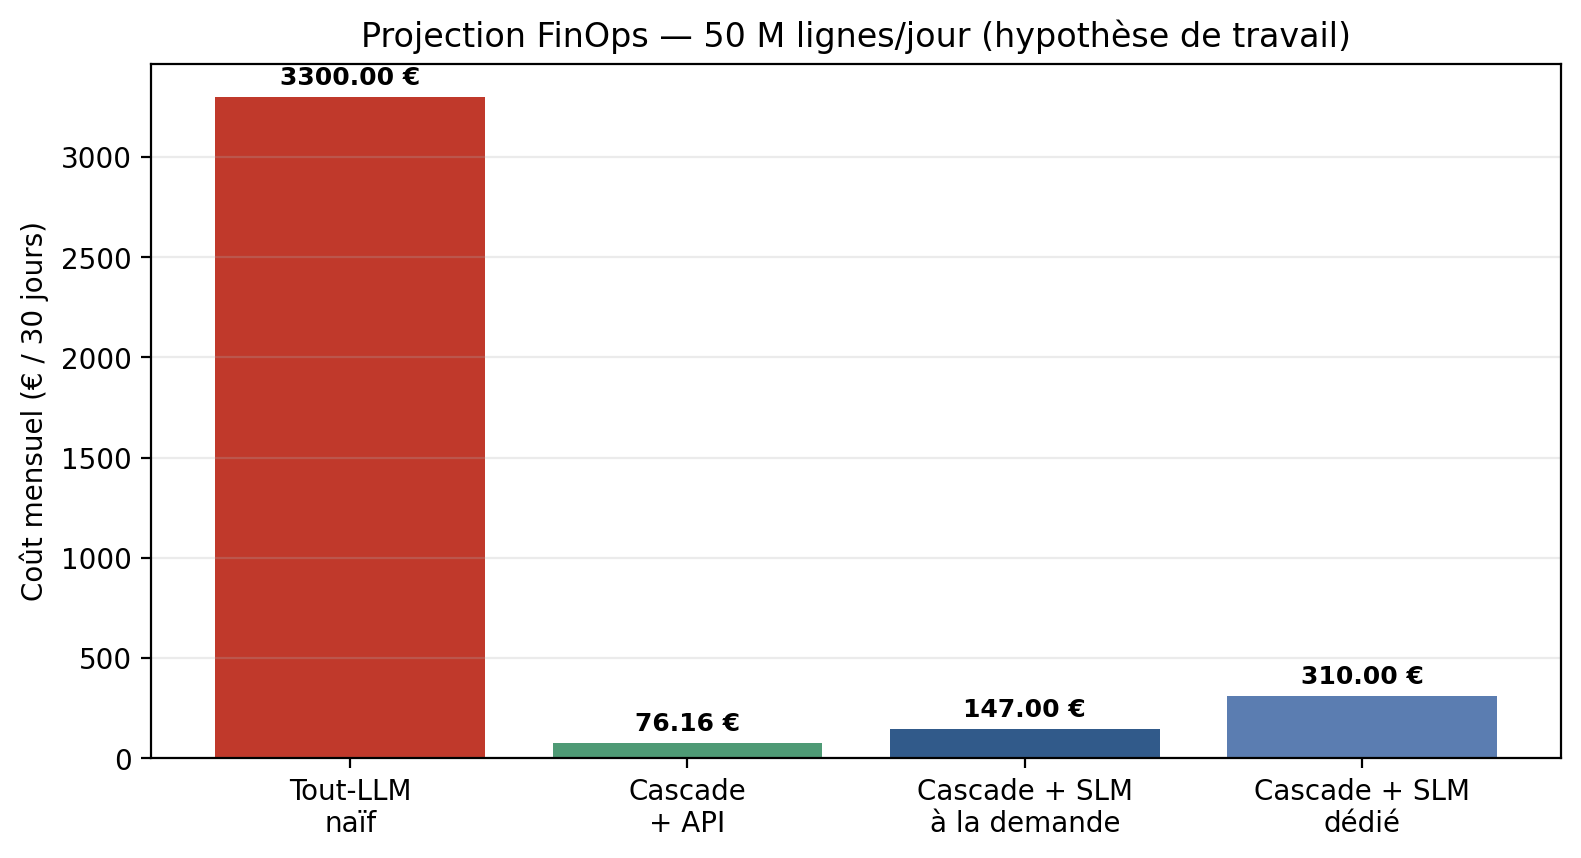
\includegraphics[width=0.9\linewidth]{fig_finops.png}
\caption{Projection mensuelle à 50~M lignes/jour : 3\,300~\texteuro\ (tout-LLM) vs 76,16~\texteuro\ (cascade+API) vs 147~\texteuro\ (cascade+SLM à la demande) vs 310~\texteuro\ (dédié).}
\label{fig:finops}
\end{figure}

Ratio naïf/hybride $\approx \times 43$. Surcoût de souveraineté $\approx$ +71~\texteuro/mois ($\times 1{,}9$) : prix de la non-sortie des données (RGPD, PCI-DSS). Seuil d'équilibre dédié vs API $\sim$785~M lignes/jour. Le SLM local (Qwen2.5-1.5B, $\sim$34,4~s/diagnostic, 8,3~h GPU/jour, 35\,\% d'occupation) n'est pas un choix de coût marginal mais de conformité.

\subsection{Risques, limites, acceptabilité}

Hallucinations neutralisées par JSON strict + catalogue fini + injection déterministe ; dérive syntaxique suivie via [UNK]. Limites : un seed, comparaison article non appariée, biais d'attribution NameNode vs DataNode (corriger par topologie cluster en contexte), évaluation HDFS à étendre au multi-services. Acceptabilité : dossier de preuves joint à chaque alerte, mode conseiller supervisé.

\section{Conclusion}

V2 verrouillée : \textbf{0,8267 / 0,8362 / 0,8314} (1~seed), ROC-AUC 0,9235, PR-AUC 0,7051, FPR 0,30\,\% sur 506\,540 sessions ; V3 BGL : \textbf{0,9045 / 0,9166 / 0,9105} (moy. 3~seeds, $\pm$0,0035 en F1), au niveau du papier BGL (90,83). L'hybridation concilie détection, explicabilité contrainte et soutenabilité ($\div 43$, 76--147~\texteuro/mois). Dépassement article partiel, à consolider multi-seeds. Recommandations : registre MLOps par profil, FinOps by design ($<$1\,000 appels/jour), boucle human-in-the-loop, mesure MTTR en double aveugle.

\begin{thebibliography}{99}
\bibitem{vaswani2017attention} Vaswani et al. Attention is all you need. NeurIPS, 2017.
\bibitem{kingma2013vae} Kingma, Welling. Auto-encoding variational Bayes. ICLR, 2013.
\bibitem{devlin2018bert} Devlin et al. BERT. NAACL, 2018.
\bibitem{he2017drain} He et al. Drain: online log parsing with fixed depth tree. ICWS, 2017.
\bibitem{guo2021logbert} Guo et al. LogBERT: log anomaly detection via BERT. IJCNN, 2021.
\bibitem{logbert-repo} Dépôt officiel LogBERT. \url{https://github.com/HelenGuohx/LogBERT.git}, commit \texttt{a845e61}.
\bibitem{zhu2019tools} Zhu et al. Tools and benchmarks for automated log parsing. ICSE-SEIP, 2019.
\bibitem{he2020loghub} He et al. Loghub: a large collection of system log datasets. ISSRE, 2020.
\bibitem{du2017deeplog} Du et al. DeepLog: anomaly detection and diagnosis from logs. CCS, 2017.
\bibitem{xu2009detecting} Xu et al. Online system problem detection by mining patterns of console logs. ICDM, 2009.
\bibitem{scholkopf2001estimating} Schölkopf et al. Estimating the support of a high-dimensional distribution. Neural Computation, 2001.
\bibitem{liu2008isolationforest} Liu et al. Isolation Forest. ICDM, 2008.
\bibitem{lin2016logcluster} Lin et al. Log clustering based problem identification for online service systems. ICSE, 2016.
\bibitem{he2016experience} He et al. Experience report: system log analysis for anomaly detection. ISSRE, 2016.
\bibitem{meng2019loganomaly} Meng et al. LogAnomaly: unsupervised detection of sequential and quantitative anomalies. IJCAI, 2019.
\bibitem{xu2010mining} Xu et al. Detecting large-scale system problems by mining console logs. SOSP, 2009.
\bibitem{ndichu2026} Ndichu et al. Alert fatigue in production supervision, 2026.
\bibitem{ji2023hallucination} Ji et al. Survey of hallucination in NLG. ACM Comp. Surv., 2023.
\bibitem{qwen2025} Qwen Team. Qwen2.5 technical report, 2025.
\bibitem{llama3} Meta AI. Llama 3 model card, 2024.
\bibitem{heaps1978} Heaps. Information retrieval. Academic Press, 1978.
\bibitem{han2022ervised} Han et al. A survey on AIOps for failure management. ACM Comp. Surv., 2022.
\bibitem{notaro2021aion} Notaro et al. AIOps: chronology, landscape and challenges. IEEE Trans. Net. Serv. Manag., 2021.
\bibitem{worldline-deu2024} Worldline. Document d'enregistrement universel 2024. Investors Worldline, chiffre d'affaires 4\,632~M\texteuro, $\sim$18\,000 experts, $\sim$40 pays. \url{https://investors.worldline.com/}.
\bibitem{worldline-site} Worldline. PayTech provider, services aux institutions financières et implantations. \url{https://worldline.com/}.
\end{thebibliography}

\end{document}